\section{An information theoretic approach}

% The problem with increasing complexity
% - Training and test loss as a function of complexity - use trees
% We seek to minimize generalization error
% Most common strategy: cross validation on different input settings
% Goal: Estimate generalization error analytically, by adjusting training error
% Specifically: Estimate generalization error for trees analytically
% Quite generally: 2cov(y_i pred_i)
% So the goal is to estimate cov
% For likelihoods: Akaike - explain Taylor approx?
% Is generalized for differentiable (in parameters) loss functions NIC (Murata)
% Does not apply directly to trees, due to the non-standard binary splitting procedure
% However, conditioned on topology. Only leaf-parameters are learned (satisfies differentiability etc.) - local optimism as NIC
% Big result - 

\begin{frame}{Revisit the supervised learning problem}
	The goal is to find $f$ that minimises \textit{generalization error}:
	\begin{align*}
	\hat{f} = \arg\min_f E_{\hat{\theta},\features^0\response^0}\left[l(\response^0,f(\features^0;\hat{\theta}))\right]
	\end{align*}
	where $(\features^0\response^0)$ are unseen in the training-phase, and therefore independent of $\hat{\theta}$ trained from $(\features,\response)$.
	
	\begin{columns}[T]
		\begin{column}{0.35\textwidth}
		\includegraphics<2->[height=4.5cm,width=4.5cm]{figures/loss_vs_complexity.pdf}			
		\end{column}
		\begin{column}{0.6\textwidth}
			\visible<3->{
			\begin{myblock}{}{bg=yellow!05,fg=black}{bg=yellow!20, fg=black}
				\begin{itemize}
					\item<1-> Optimism of the training loss: \small$$C(\hat{\theta}) = E\left[l(\response^0,f(\features^0;\hat{\theta})) - l(\response,f(\features;\hat{\theta}))\right]$$
					\item<1-> Often \small$C(\hat{\theta})\approx \frac{2}{n}\sum_{i=1}^n\Cov(y_i,\pred_i)$
					\item<1-> Useful to talk about \textit{asymptotic loss} \small$$E\left[l(\response,f(\features;\theta_0))\right],~\lim_{n\to\infty}\hat{\theta}\stackrel{P}{\to}\theta_0$$
				\end{itemize}
			\end{myblock}}
		\end{column}
	\end{columns}
	
	
%	The goal is to find $f$ that minimizes generalization error:
%	
%	where XXX is data unseen in the training-phase.
%	
%	Training and test error on as a function of complexity
%	
%		Optimism definition
%	
%	Then add asymptotic one
%	
%	The general result with cov
	
	
\end{frame}

\begin{frame}{But the ensemble complexity is unknown...}
	
	\begin{myblock}{The main idea:}{bg=green!05,fg=black}{bg=green!20, fg=black}
		\begin{itemize}
			\item<1-> Estimate $C(\hat{\theta})$ for trees analytically!
		\end{itemize}
	\end{myblock}
	
	\begin{myblock}{And hope that we may...}{bg=yellow!05,fg=black}{bg=yellow!20, fg=black}
		\begin{enumerate}
			\item<2-> Adaptively control the complexity of each tree
			\item<3-> Automatically stop the boosting procedure
			%\item<4-> In a highly efficient manner
		\end{enumerate}
	\end{myblock}
	\begin{columns}[T]
	\begin{column}{0.35\textwidth}
		% tree loss vs depth
		\includegraphics<2->[height=4cm,width=4.5cm]{figures/loss_vs_treedepth1.pdf} 
	\end{column}
	\begin{column}{0.35\textwidth}
		% no split at all
		\includegraphics<3>[height=4cm,width=4.5cm]{figures/loss_vs_treedepth2.pdf}
	\end{column}
	\end{columns}
	
\end{frame}

\begin{frame}{Information criteria: Akaike and beyond...}
	\begin{myblock}{The poor researcher has no processing power...}{bg=blue!5,fg=black}{bg=blue!10, fg=black}
		\begin{itemize}
			\item<1-> An analytic, not a data-driven approach, is needed!
		\end{itemize}
	\end{myblock}
	\visible<2->{\begin{myblock}{A brief history of (some) information criteria}{bg=yellow!05,fg=black}{bg=yellow!20, fg=black}
		\begin{itemize}
			\item<2-> \cite{akaike1974new} AIC: $C=p$ for NLL. Assumptions on true model
			\item<2-> \cite{takeuchi1976distribution} TIC: $C = \tr(QH^{-1})$ also for NLL, but no assumption on the true model
			\item<2-> \cite{murata1994network} NIC: $C = \tr(QH^{-1})$ also for differentiable loss
		\end{itemize}
		\begin{align*}
	H&=\E \left[ \nabla_{\mathbf{\theta}_0}^2 \loss(\response,f(\features;\mathbf{\theta}_0)) \right]\\ 
	Q &= \E\left[ \left( \nabla_{\theta_0}\loss(\response,f(\features;\mathbf{\theta}_0)) \right)\left( \nabla_{\theta_0}\loss(\response,f(\features;\mathbf{\theta}_0)) \right)^\intercal  \right]
	\end{align*}
	\end{myblock}
}
	%Yellow block local optimism conditioning?
\end{frame}

\begin{frame}{The local optimism}
	
				\begin{myblock}{But can we use this for trees?}{bg=blue!5,fg=black}{bg=blue!10, fg=black}
				\begin{itemize}
					\item<2-> Conditionally on known tree-topology / regions $R$
					\item<2-> We define the local optimism for a leaf node $t$
					\begin{align*}
						\mathcal{C}(t|q) &= 
						\E_{y,\hat{w}_t} \left[ \frac{\partial^2}{\partial \hat{w}_t^2}\tilde l(\response,\hat{w}_t)\right]
						\Var_{\hat{w}_t}[\hat{w}_{t}]
					\end{align*}
					$q$ is the tree-topology, $\hat{w}_t$ is the prediction in region $t$
				\end{itemize}
			\end{myblock}
		
		\visible<3->{
	\begin{myblock}{Correspondingly for internal nodes...}{bg=yellow!05,fg=black}{bg=yellow!20, fg=black}
		\begin{itemize}
			\item<3-> At some stage in the tree building process every node will have been a leaf node.
			\item<3-> Define this to be the local optimism $\mathcal{C}(t|q)$ for the internal node $t$ in the fully grown tree.
		\end{itemize}
	\end{myblock}	
	}			

\end{frame}

\begin{frame}{The local optimism: Illustration}
	\centering\resizebox{7cm}{4cm}{
		\begin{tikzpicture}
\tikzstyle{custbox} = [circle, align=left, minimum width=0.5cm, minimum height=0.5cm,text centered, draw=black, fill=gray!10]

\node (r) at (0,0) [custbox]{1}; 
\node[right=0.2cm of r] (optimismr) {$\mathcal{C}(1|q_1)$};

\node (rl) at (-1.5,-1.5) [custbox]{2}; 
\node[left=0.2cm of rl] (optimismrl) {$\mathcal{C}(2|q_2)$};

\node (rll) at (-2.5,-3) [custbox]{4}; \node[below left=0.2cm and 0cm of rll] (opt4) {$\mathcal{C}(4|q_4)$}; 
\node (rlr) at (-0.5,-3) [custbox]{5}; \node[below left=0.2cm and 0cm of rlr] (opt5) {$\mathcal{C}(5|q_5)$}; 

\node (rr) at (1.5,-1.5) [custbox]{3};
\node[right=0.2cm of rr] (optimismrr) {$\mathcal{C}(3|q_3)$};

\node (rrl) at (0.5,-3) [custbox]{6};
\node[below right=1cm and 1cm of rrl] (optimismrrl) {$\mathcal{C}(6|q_6)$};

\node (rrll) at (0,-4.5) [custbox]{8}; \node[below left=0.2cm and 0cm of rrll] (opt8) {$\mathcal{C}(8|q_8)$}; 
\node (rrlr) at (1,-4.5) [custbox]{9}; \node[below right=0.2cm and 0cm of rrlr] (opt9) {$\mathcal{C}(9|q_9)$}; 
\node (rrr) at (2.5,-3) [custbox]{7}; \node[below right=0.2cm and 0cm of rrr] (opt7) {$\mathcal{C}(7|q_7)$}; 

%Arrows
\draw[->,black] (r) -- (rl);
\draw[->,black] (r) -- (rr);
\draw[->,black] (rl) -- (rll);
\draw[->,black] (rl) -- (rlr);
\draw[->,black] (rr) -- (rrl);
\draw[->,black] (rr) -- (rrr);
\draw[->,black] (rrl) -- (rrll);
\draw[->,black] (rrl) -- (rrlr);
%optimism
\draw[-,orange] (r) -- (optimismr);
\draw[-,orange] (rr) -- (optimismrr);
\draw[-,orange] (rrl) -- (optimismrrl);
\draw[-,orange] (rl) -- (optimismrl);
\draw[-,orange] (rll) -- (opt4);
\draw[-,orange] (rlr) -- (opt5);
\draw[-,orange] (rrr) -- (opt7);
\draw[-,orange] (rrll) -- (opt8);
\draw[-,orange] (rrlr) -- (opt9);


\end{tikzpicture}
}

The optimism induced from fitting the predictions $\mathbf{w}$ in the leaf-nodes conditioned on the final topology is given as
\begin{align*}
	\hat{C}(\hat{\mathbf{w}}|q) = \sum_{t\in\{4,5,8,9,7\} } \mathcal{C}(t|q)\pi_t,~\pi_t=P(q(\mathbf{x})=t)
\end{align*}

\end{frame}


\begin{frame}{The tree-learning procedure learns the future map $q$}
	\begin{myblock}{The steps - first consider only one feature}{bg=blue!5,fg=black}{bg=blue!10, fg=black}
	\begin{itemize}
		\item<1-> Relate the distance between the training and asymptotic loss to a gamma distribution
		\item<1-> Fit the gamma using knowledge of its shape and expectation
	\end{itemize}
	\end{myblock}
\visible<2->{
	\begin{myblock}{The steps - consider $m\geq 1$ features}{bg=yellow!05,fg=black}{bg=yellow!20, fg=black}
		\begin{itemize}
			\item<2-> Under $H_0$: no feature is relevant
			\item<2-> Distance between training and asymptotic loss as expected maximum of multiple realizations of the gamma RV
		\end{itemize}
	\end{myblock}	
}	
\begin{itemize}
	\item<2-> Warning: several approximations!
\end{itemize}
\end{frame}

\begin{frame}{Gives the following result:}
	\begin{align*}
	\hat{C}_m(\hat{\mathbf{w}}, q) 
	=
	2 \sum_{t\not\in \mathcal{L}} \E \left[
	Q\left(
	d(t), \frac{ \mathcal{C}(L(t)|q)\pi_{L(t)} + \mathcal{C}(R(t)|q)\pi_{R(t)} }{2}, m
	\right)
	\right]
	\end{align*}
	\begin{itemize}
		\item $\mathcal{L}$ is the set of leaf nodes
		\item $Q(\alpha,\beta,m)$ is the maximum of $m$ gamma random variables with shape $\alpha$ and scale $\beta$
		\item $L(t)$ and $R(t)$ returns the index of left and right child-nodes respectively
		\item 	\small\begin{align*}
		d(t) = 
		\begin{cases}
		3 & \text{if } L(t) \in \setleafnodes \text{ and } R(t) \in \setleafnodes\\
		\frac{5}{2} & \text{if } L(t) \in \setleafnodes \text{ and } R(t) \not\in \setleafnodes\\
		\frac{5}{2} & \text{if } L(t) \not\in \setleafnodes \text{ and } R(t) \in \setleafnodes\\
		2 & \text{if } L(t) \not\in \setleafnodes \text{ and } R(t) \not\in \setleafnodes.
		\end{cases}
		\end{align*} 
	\end{itemize}
\end{frame}

\begin{frame}{Visualization of the result}
	\centering\resizebox{11cm}{4.5cm}{
	\begin{tikzpicture}
	\tikzstyle{custbox} = [circle, align=left, minimum width=0.5cm, minimum height=0.5cm,text centered, draw=black, fill=gray!10]
	
	\node (r) at (0,0) [custbox]{1}; 
	\node[right=0.2cm of r] (optimismr) {$2E\left[Q\left(2,\frac{\mathcal{C}(2|q)\pi_2+\mathcal{C}(3|q)\pi_3}{2}, m\right)\right]$};
	
	\node (rl) at (-1.5,-1.5) [custbox]{2}; 
	\node[left=0.2cm of rl] (optimismrl) {$2E\left[Q\left(3,\frac{\mathcal{C}(4|q)\pi_4+\mathcal{C}(5|q)\pi_5}{2}, m\right)\right]$};
	
	\node (rll) at (-2.5,-3) [custbox]{4}; %\node[below=0.2cm of rll] {$\hat{w}_1$}; 
	\node (rlr) at (-0.5,-3) [custbox]{5}; %\node[below=0.2cm of rlr] {$\hat{w}_2$}; 
	
	\node (rr) at (1.5,-1.5) [custbox]{3};
	\node[right=0.2cm of rr] (optimismrr) {$2E\left[Q\left(\frac{5}{2},\frac{\mathcal{C}(6|q)\pi_6+\mathcal{C}(7|q)\pi_7}{2}, m\right)\right]$};
	
	\node (rrl) at (0.5,-3) [custbox]{6};
	\node[below right=1cm and 1cm of rrl] (optimismrrl) {$2E\left[Q\left(3,\frac{\mathcal{C}(8|q)\pi_8+\mathcal{C}(9|q)\pi_9}{2}, m\right)\right]$};
	
	\node (rrll) at (0,-4.5) [custbox]{8};% \node[below=0.2cm of rrll] {$\hat{w}_3$}; 
	\node (rrlr) at (1,-4.5) [custbox]{9};% \node[below=0.2cm of rrlr] {$\hat{w}_4$}; 
	\node (rrr) at (2.5,-3) [custbox]{7}; %\node[below=0.2cm of rrr] {$\hat{w}_5$}; 
	
	%Arrows
	\draw[->,black] (r) -- (rl);
	\draw[->,black] (r) -- (rr);
	\draw[->,black] (rl) -- (rll);
	\draw[->,black] (rl) -- (rlr);
	\draw[->,black] (rr) -- (rrl);
	\draw[->,black] (rr) -- (rrr);
	\draw[->,black] (rrl) -- (rrll);
	\draw[->,black] (rrl) -- (rrlr);
	%optimism
	\draw[-,orange] (r) -- (optimismr);
	\draw[-,orange] (rr) -- (optimismrr);
	\draw[-,orange] (rrl) -- (optimismrrl);
	\draw[-,orange] (rl) -- (optimismrl);
	
	\end{tikzpicture}
}
	\begin{itemize}
	\item Sum up the node-contributions to obtain the optimism estimate
	\end{itemize}
\end{frame}

\begin{frame}{Estimation}
	Quantities must admit evaluation and efficient computation:
	\begin{itemize}
		\item<2-> Conditioned on $q$, $\hat{\mathbf{w}}$ are M-estimators.
		\item<2-> 	\begin{align*}
		\lim_{n\to\infty}
		\mathcal{C}(t|q)\pi_t
		&=
		\E_{y,\hat{w}_t} \left[ \frac{\partial^2}{\partial \hat{w}_t^2}l(\response,\hat{w}_t)\right]
		\Var_{\hat{w}_t}[\hat{w}_{t}]\pi_t\\
		%,~t\in\setleafnodes,~q(\features)=t\\
		&= 
		\frac{\sum_{i\in I_t} \left(g_i+h_i\hat{w}_t\right)^2}{n\sum_{i\in I_t}h_i},
		\text{ $I_t$ is indexes of obs in leaf $t$}
		\end{align*}
		\item<3-> Assume features independent, then $E[Q]$ is the expected $m-$th order statistic
		\item<3-> Estimate asymptotically using the gamma-quantile function: $$E[Q]\sim z\left(\frac{m}{m+1}\right)$$
	\end{itemize}
\end{frame}

\begin{frame}{Some sanity checks: Simulation experiments}
	
	100 Datasets and 100 trees, trained on 1 and 100 features.
		\begin{figure}[h]
		\centering
		\begin{subfigure}{.43\textwidth}
			\centering
			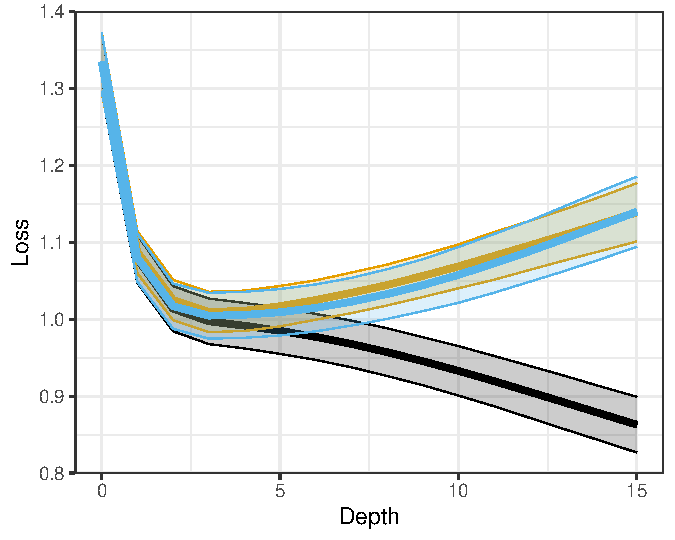
\includegraphics[scale=0.4]{figures/loss_vs_depth_one_feature.pdf}
			\caption[]{One (relevant) feature}
			\label{fig: loss vs tree depth one feature}
		\end{subfigure}
		\begin{subfigure}{.53\textwidth}
			\centering
			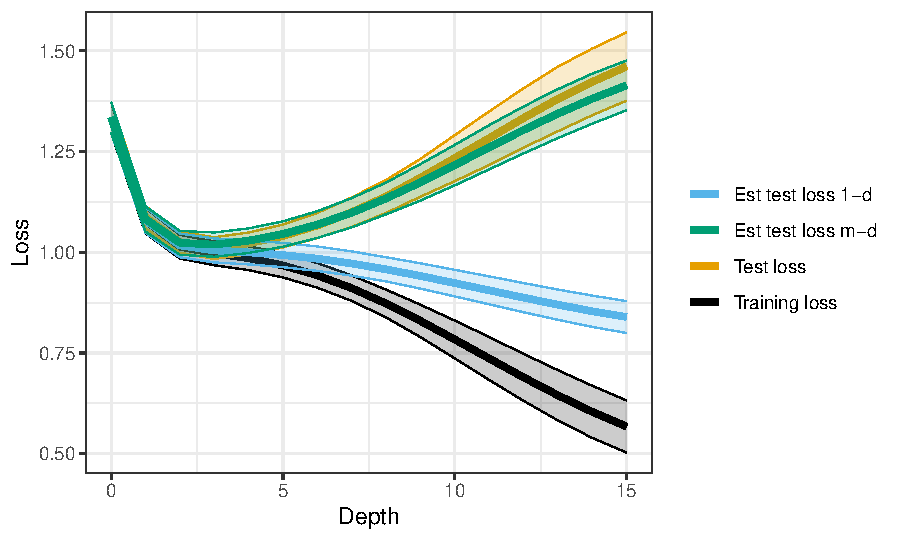
\includegraphics[scale=0.4]{figures/loss_vs_depth_dim_correct.pdf} 
			\caption[]{100 features of which 99 are noise}
			\label{fig: loss vs tree depth multiple feature}
		\end{subfigure}
	\caption{Average $\pm 2 SD$ for training (black) and test (orange) MSE loss, together with estimated optimism (blue: 1 feature, green: 100 features)}
		%\caption{The average $\pm 2 SD$ for training (black) and test (orange) MSE loss, and estimated optimism, after training on 100 simulated datasets, each containing 10000 realizations from a linear model $y\sim N(x,1)$ where $x\sim U(0,2)$. In Figure (a), training is done on only one feature (the relevant $x$), and the quantity \eqref{eq:expected tree optimism one feature} (blue) is the optimism added to the training loss. Figure (b) results from the same data and training, but with 99 added Gaussian noise features. Resulting is that the optimism from Figure (a) is pushed downwards, and in need of the correction given in \eqref{eq:optimism full m} (green). }
	\end{figure}
	\begin{itemize}
		\item<2-> Not crazy!
	\end{itemize}
\end{frame}
